%%%%%%%%%%%%%%%%%%%%%%%%%%%%%%%%%%%%%%%%%%%%%%%%%%%%%%%%%%%%%%%%%%%%%
%% FELP manuscript draft
%% JCTC submission (achemso)
%%%%%%%%%%%%%%%%%%%%%%%%%%%%%%%%%%%%%%%%%%%%%%%%%%%%%%%%%%%%%%%%%%%%%
\documentclass[journal=jctcce,manuscript=article,layout=twocolumn,hyperref=true]{achemso}

\usepackage{graphicx}
\usepackage{microtype}
\usepackage{amsmath}

\makeatletter
\renewcommand{\@seccntformat}[1]{\csname the#1\endcsname.\quad}
\makeatother

\captionsetup[figure]{labelfont=bf,textfont=rm,labelsep=period}
\captionsetup[figure*]{labelfont=bf,textfont=rm,labelsep=period}

\newcommand{\figref}[2][]{\textbf{Figure~\ref{#2}#1}}
\newcommand{\figrefp}[2][]{\textbf{(Figure~\ref{#2}#1)}}
\newcommand{\figsref}[2]{\textbf{Figures~\ref{#1} and~\ref{#2}}}
\newcommand{\figsrefp}[2]{\textbf{(Figures~\ref{#1} and~\ref{#2})}}
\newcommand{\figsrefc}[2]{\textbf{Figures~\ref{#1},~\ref{#2}}}
\newcommand{\figsrefcp}[2]{\textbf{(Figures~\ref{#1},~\ref{#2})}}
\newcommand{\figrefcap}[2][]{Figure~\ref{#2}#1}
\newcommand{\eqnref}[1]{eq~\ref{#1}}

\title{Free Energy Landscape Perturbation for Estimating Mutation-Induced Population Shifts from Reference Molecular Dynamics Ensembles}
\author{Tatum E. Murdock}
\affiliation{Chemical and Physical Biology Program, Vanderbilt University, Nashville, Tennessee 37232, United States}
\alsoaffiliation{Center for AI in Protein Dynamics, Vanderbilt University, Nashville, Tennessee 37232, United States}
\author{Benjamin P. Brown}
\email{benjamin.p.brown@vanderbilt.edu}
\affiliation{Department of Pharmacology, Vanderbilt University, Nashville, Tennessee 37232, United States}
\alsoaffiliation{Center for AI in Protein Dynamics, Vanderbilt University, Nashville, Tennessee 37232, United States}

\begin{document}

\begin{abstract}
		Mutations can alter protein function by redistributing probability among conformational states, even when structural changes are modest. Directly estimating a perturbed conformational free energy landscape with molecular dynamics is expensive because each mutation requires a new converged simulation. Here, we introduce Free Energy Landscape Perturbation (FELP), a state-local reweighting framework that estimates mutation-induced population shifts from a reference ensemble. FELP partitions a reference trajectory into discrete microstates, evaluates restrained reference-to-perturbed energy differences for configurations sampled within each state, and combines spatially regularized state-local Zwanzig factors with the reference state probabilities to estimate the perturbed state distribution. FELP estimates how a perturbation changes the relative probabilities of conformational basins and reports effective-sample and overlap diagnostics that identify when the predicted shift lacks support in the sampled reference ensemble. We describe the FELP estimator, its implementation, and its performance on glycine dipeptide, chignolin, and T4 lysozyme. FELP is intended for perturbations that reshape populations within a sufficiently sampled reference landscape, providing a practical bridge between local alchemical energy evaluation and ensemble-level mechanistic interpretation.
\end{abstract}

	\section{Introduction}

	The functional repertoire of a protein is fundamentally determined by its conformational free energy landscape. Folding, stability, enzyme catalysis, signal transduction, molecular recognition, and allosteric regulation all depend on how probability is distributed over conformational states and how readily the system moves between them. Many proteins therefore function through ensembles of native-like substates, with activity controlled by changes in basin depth, transition pathways, and relative occupancy. Quantitatively describing these landscapes is central to understanding how sequence, ligand binding, protonation, and chemical modification alter biological function.

	Molecular dynamics (MD) simulations provide a direct route to estimating these conformational free energy landscapes at atomistic resolution. In principle, sufficiently long trajectories recover both the relevant structural diversity and the thermodynamic probability of each state. In practice, sampling remains the central limitation. Transitions between functional conformations can be slow, rare, and system-specific, such that converging a separate MD ensemble for every perturbation of interest is often prohibitively expensive. Parallel simulation strategies, enhanced sampling methods such as replica exchange \cite{sugita1999replica} and metadynamics \cite{laio2002metadynamics}, and Markov state models (MSMs) \cite{chodera2014msm,husic2018msm} have improved access to long-timescale behavior by combining many trajectories into kinetic and thermodynamic state models. However, even with these advances, each new mutation or chemical change can still demand substantial additional sampling to converge a new landscape. This expense is a principal bottleneck for systematic structure--function studies that require evaluating many perturbations against a shared conformational baseline.

	To avoid the cost of full ensemble resampling, computational methods often sacrifice conformational diversity for speed. Single-structure and local relaxation methods, such as Rosetta $\Delta\Delta G$ estimates for mutation stability calculations, can test whether a particular coordinate set becomes more or less favorable after mutation, but they typically evaluate a narrow structural hypothesis \cite{kellogg2011rosetta}. Minimal relaxation avoids the cost of full resampling, yet it can convert small coordinate differences into abrupt energy changes and noisy estimates. These calculations can be useful for local stability screening, but they generally do not directly answer whether a mutation stabilizes one conformational basin over another.

	Alchemical methods such as free energy perturbation (FEP) provide a formally rigorous extension of this idea. By computing free energy differences between Hamiltonians from local equilibrium samples, FEP incorporates local flexibility and avoids the abrupt energy changes of single-structure minimization \cite{zwanzig1954fep,lu2001fepaccuracy,shirts2005comparison,pohorille2010freeenergy,shirts2008mbar,klimovich2015guidelines,he2018alchemical}. However, practical protein mutation calculations remain structurally restricted because they are initialized from a small number of conformations and restrained to prevent structural drift. Both single-structure screening and local FEP calculations estimate the energetic effect of a perturbation in a specific structural context. Additional ensemble analysis is required to describe how that perturbation redistributes probability across a complex conformational landscape. Furthermore, exponential free energy estimators rely heavily on the assumption that the reference and target states share sufficient phase-space overlap \cite{wu2005overlap1,wu2005overlap2}. Because these estimators are highly sensitive to rare and high-weight samples, inadequate overlap can produce unstable estimates that appear numerically converged but are driven by too few configurations.

	Recent population-shift strategies address this ensemble problem by separating conformational sampling from perturbation evaluation. This approach originally emerged in the context of ligand binding to quantify conformational selection and induced-fit mechanisms. Implicit-ligand theory, for example, provides a rigorous analytical framework for estimating how a binding event reweights host conformations without requiring explicit simulation of the bound complex \cite{minh2012implicit,nguyen2018implicit,schutte2015alchemy}. While traditional implicit-ligand theory typically evaluates these shifts using exact volume integrals or analytical interaction potentials over a continuous ensemble, recent methods adapt this logic to discrete kinetic models and empirical scoring. PopShift, for instance, evaluates discrete ligand docking scores against the states of a ligand-free MSM to predict binding-induced population shifts \cite{smith2024popshift}. The unifying insight of these approaches is that expensive sampling can be performed once for a reference system. Once the reference state probabilities are established, the effects of many different ligands can be evaluated against the same conformational baseline. This framework moves beyond single-structure scoring by explicitly linking the energetic preference of a perturbation to the thermodynamic weight of each conformational state.

	Here, we introduce Free Energy Landscape Perturbation (FELP) to apply this population-shift framework to amino acid mutations. FELP combines a sampled reference ensemble, discrete state models, restrained local perturbation evaluation, and FEP-style reweighting. The method partitions a reference ensemble into discrete microstates, evaluates the energetic effect of a mutation within each state, and reweights the reference probabilities to estimate how the mutation redistributes probability over the pre-sampled landscape. By treating a global population shift as a collection of tractable local reweighting problems, FELP bridges the gap between single-structure scoring and full-ensemble resampling. To address the inherent phase-space overlap limitations of exponential estimators, FELP explicitly audits its predictions using effective sample size and weight-concentration diagnostics \cite{lyman2007ess,zhang2010ess}. These diagnostics ensure that the method not only predicts how a mutation reshapes a landscape but also identifies when a proposed perturbation requires conformations that were not adequately sampled by the reference ensemble.

	\section{Theory}

	Consider a reference system with potential energy $U_0(x)$ and a perturbed system with potential energy $U_1(x)$, where $x$ denotes a molecular configuration and $\beta = (k_B T)^{-1}$. The Boltzmann distribution maps these potential energy functions to continuous probability densities over configurations. FELP starts from a sampled reference ensemble, such as an MD trajectory or another state model with a meaningful reference prior, that represents configurations drawn from the reference distribution $p_0(x) \propto \exp[-\beta U_0(x)]$. FELP partitions this configuration space into discrete microstates $i \in \{1,\ldots,N\}$ using a chosen collective variable or feature representation. Let $\chi_i(x)$ be the indicator function for state $i$. The restricted partition function for state $i$ under Hamiltonian $a$ is
\begin{equation}
		Z_a(i) = \int \chi_i(x)\exp[-\beta U_a(x)]\,dx,
\end{equation}
	and the corresponding thermodynamic probability of the microstate is $\pi_a(i) = Z_a(i)/\sum_k Z_a(k)$. For the reference system, this is equivalent to integrating the continuous reference density over the microstate to obtain the reference prior $\pi_0(i)$. FELP aims to estimate the perturbed microstate probabilities $\pi_1(i)$ using only samples drawn from the reference ensemble \figrefp{fig:FELPWorkflow}.
	
	\begin{figure*}[t]
		\centering
		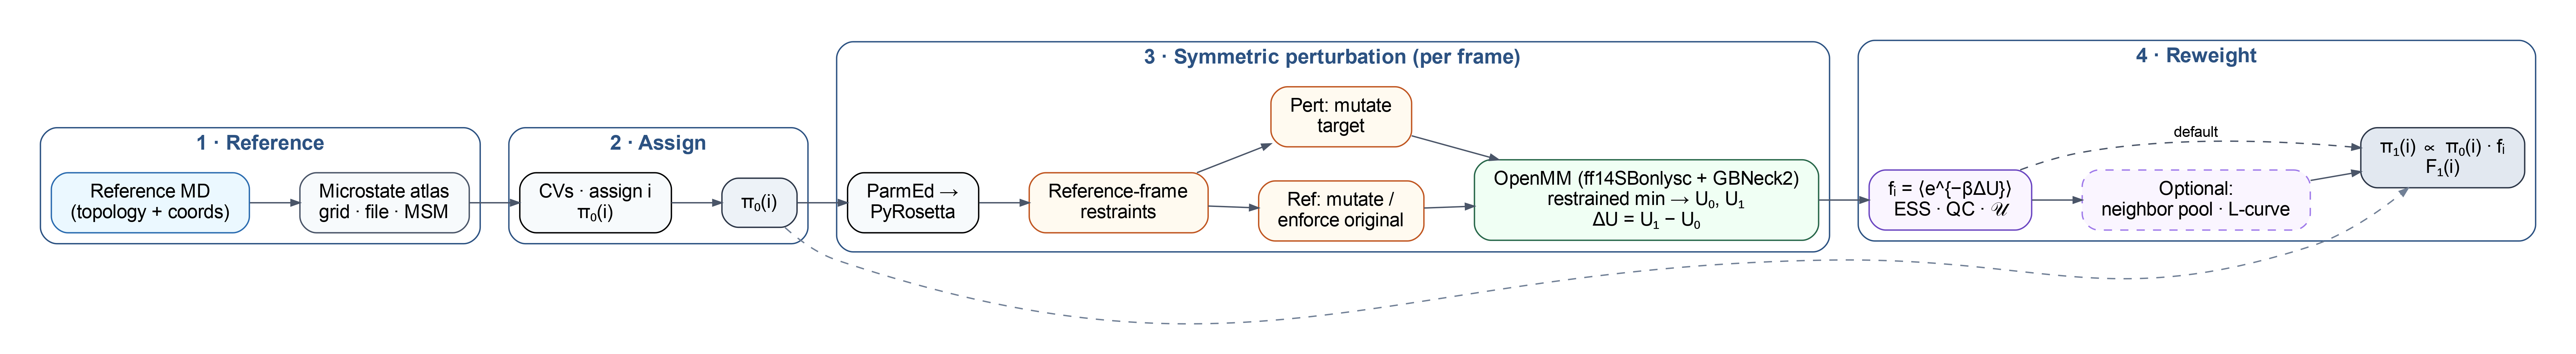
\includegraphics[width=\textwidth]{figures/felp_workflow_schematic_wide.png}
		\caption{\textbf{Free Energy Landscape Perturbation workflow.} FELP begins from a sampled reference ensemble and a microstate atlas, assigns configurations to obtain the reference prior $\hat{\pi}_0(i)$, and evaluates symmetric reference and perturbed branches under reference-frame restraints. The default OpenMM reweighting Hamiltonian uses ff14SB sidechain-only parameters with GBNeck2 implicit solvent to compute $\Delta U=U_1-U_0$ for each evaluated configuration. State-local Zwanzig factors are combined with $\hat{\pi}_0(i)$ to estimate $\hat{\pi}_1(i)$ and $F_1(i)$; optional neighbor pooling can regularize noisy local estimates before normalization.}
		\label{fig:FELPWorkflow}
	\end{figure*}
	
	To bridge the reference and perturbed ensembles, FELP relies on the principle that global conformational shifts can be decomposed into local reweighting problems. Within a specific microstate, the ratio of restricted partition functions follows the two-state Zwanzig identity,
\begin{equation}
		\frac{Z_1(i)}{Z_0(i)}
		=
		\left\langle \exp[-\beta \Delta U(x)] \right\rangle_{0,i},
		\label{eq:restricted_zwanzig}
\end{equation}
	where $\Delta U(x)=U_1(x)-U_0(x)$ and $\left\langle \cdot \right\rangle_{0,i}$ denotes an ensemble average over reference configurations conditioned on membership in state $i$. Normalizing the restricted partition functions over all microstates yields the central FELP estimator:
\begin{equation}
		\pi_1(i) =
		\frac{\pi_0(i)\left\langle \exp[-\beta \Delta U(x)] \right\rangle_{0,i}}
		{\sum_k \pi_0(k)\left\langle \exp[-\beta \Delta U(x)] \right\rangle_{0,k}}.
	\label{eq:state_reweighting}
\end{equation}
	Equation~\ref{eq:state_reweighting} preserves the reference state decomposition and updates the probability of each state according to the perturbation's energetic effect on configurations sampled within that specific state.
	
	The central hypothesis behind this formulation is that discretization creates domains of local phase-space overlap. By conditioning the exponential average on microstate membership, FELP assumes that reference configurations assigned to state $i$ adequately represent the structural ensemble of the perturbed system within that same state. FELP evaluates the perturbation directly from the reference ensemble without simulating the target state or intermediate alchemical windows. If a mutation is unfavorable in one conformational basin but favorable in another, the state-local reweighting factors will predict a population shift between those basins.
	
	In a finite trajectory, state $i$ contains evaluated configurations $x_{ij}$ for $j=1,\ldots,n_i$. FELP estimates the local Zwanzig factor by computing
	\begin{equation}
		f_i = \frac{1}{n_i}\sum_{j=1}^{n_i} w_{ij},
		\qquad
		w_{ij}=\exp[-\beta(\Delta U_{ij}-s)],
	\end{equation}
	where $s=\min(\Delta U)$ over all frames included in reweighting is a uniform stability shift that prevents numerical overflow. Because this shift is applied globally, it cancels during normalization. The sample estimator of \eqnref{eq:state_reweighting} substitutes the empirical reference prior $\hat{\pi}_0(i)$ and the finite-sample factor $f_i$ for their theoretical counterparts:
	\begin{equation}
		\hat{\pi}_1(i) =
		\frac{\hat{\pi}_0(i) f_i}
		{\sum_k \hat{\pi}_0(k) f_k}.
		\label{eq:sample_reweighting}
	\end{equation}
	The corresponding relative free energy of each state is
	\begin{equation}
		F_1(i) = -k_B T \ln \hat{\pi}_1(i) + C,
	\end{equation}
	where $C$ is chosen so that the lowest finite state free energy is set to zero.
	
	Now, for finite samples, $f_i$ can be dominated by a small number of high-weight frames even when $n_i$ is large. The local effective sample size,
	\begin{equation}
		\mathrm{ESS}_i = \frac{\left(\sum_j w_{ij}\right)^2}{\sum_j w_{ij}^2},
	\end{equation}
	quantifies this weight degeneracy \cite{kong1992importance,elvira2022ess}. Low $\mathrm{ESS}_i$ indicates that the local Zwanzig factor depends on too few configurations to be reliable.
	
	Configuration space overlap requirements in unidirectional reweighting are fundamentally asymmetric. The reference ensemble must encompass the relevant configurations of the target ensemble, but the reverse is not true. It is expected that a broad reference trajectory will explore conformational states that become energetically forbidden or highly unfavorable upon perturbation. In these states, the local perturbation factor may have a low effective sample size (low $\mathrm{ESS}_i$), but this lack of samples is inconsequential if the target probability $\hat{\pi}_1(i)$ in those states is vanishingly small. The reweighted landscape remains credible as long as the states that actually carry significant target probability are adequately sampled by the reference. However, because it is rarely known \textit{a priori} whether the reference trajectory is sufficiently broad to cover all energetically relevant regions of the target ensemble, it is critical to explicitly quantify when the estimate relies on unsupported configurations. FELP therefore summarizes the validity of the reweighting operation by measuring the target probability mass assigned to unreliable states,
	\begin{equation}
		\mathcal{U} =
		\sum_i \hat{\pi}_1(i)\,
		\mathbf{1}\{\mathrm{ESS}_i < \epsilon_i\},
		\label{eq:unreliable_mass}
	\end{equation}
	where $\epsilon_i$ is an effective-sample floor for state $i$. Small $\mathcal{U}$ means the predicted landscape rests on states with adequate local sampling; large $\mathcal{U}$ is a direct reason for caution.
	
	A separate practical issue arises from discretization. The potential energy functions $U_0$ and $U_1$ are continuous, so the true restricted partition functions of neighboring microstates should vary smoothly within a basin. Treating every microstate independently forces states with low $\mathrm{ESS}_i$ to produce local factors that fluctuate sharply relative to their neighbors. FELP can optionally regularize these estimates by pooling information across adjacent states in the feature-space topology. For state $i$, the pooled factor over eligible neighboring states $\mathcal{N}(i)$ is
	\begin{equation}
		\bar{f}_i =
		\frac{\sum_{j \in \mathcal{N}(i)} \mathrm{ESS}_j\, f_j}
		{\sum_{j \in \mathcal{N}(i)} \mathrm{ESS}_j},
	\end{equation}
	with $\bar{f}_i=f_i$ when no eligible neighbors are available. The blended factor used for reweighting is
	\begin{equation}
		f_i^{\mathrm{blend}} =
		\alpha_i f_i + (1-\alpha_i)\bar{f}_i,
		\qquad
		\alpha_i = \frac{\mathrm{ESS}_i}{\mathrm{ESS}_i + \tau}.
		\label{eq:neighbor_blend}
	\end{equation}
	States with high $\mathrm{ESS}_i$ retain their local factors ($\alpha_i \approx 1$); states with low $\mathrm{ESS}_i$ borrow strength from better-sampled neighbors. \eqnref{eq:sample_reweighting} can be evaluated with $f_i^{\mathrm{blend}}$ in place of the raw $f_i$. The blending rule is therefore a shrinkage estimator wherein $\mathrm{ESS}_i$ determines how strongly the state-local estimate is trusted, while $\tau$ sets the effective-sample scale at which neighborhood information is discounted. This preserves well-sampled local perturbation factors while damping isolated fluctuations in poorly sampled states.
	
	When $\tau$ is not specified, FELP selects it by an L-curve criterion \cite{hansen1993lcurve}, balancing fidelity to the state-local estimates against smoothness over neighboring states. The fidelity term is evaluated in log-factor space,
	\begin{equation}
		\mathcal{M}(\tau) =
		\sum_i \mathrm{ESS}_i \left[\ln f_i - \ln f_i^{\mathrm{blend}}(\tau)\right]^2,
	\end{equation}
	so that well-sampled states anchor the fit and deviations are measured on the scale of local free energy corrections. The corresponding graph-smoothness penalty is
\begin{equation}
		\begin{aligned}
			\mathcal{R}(\tau) =
			\frac{1}{2}
			\sum_{i}
			\sum_{j \in \mathcal{N}(i)}
			&\left[
			\ln f_i^{\mathrm{blend}}(\tau)
			\right.\\
			&\left.
			{} - \ln f_j^{\mathrm{blend}}(\tau)
			\right]^2 .
		\end{aligned}
\end{equation}
	The selected $\tau$ is the corner of the $\mathcal{M}$--$\mathcal{R}$ curve in log--log space, defined as the point farthest from the chord connecting the two extremes. Importantly, while this regularization stabilizes noisy local factors on a discretized landscape, it does not compensate for reference conformations that were not sampled; $\mathcal{U}$ remains the primary validity criterion.
	
	\section{Results}

	\subsection{Glycine dipeptide}

	We first evaluated FELP on capped dipeptides, where the relevant conformational changes are visible directly in backbone Ramachandran ($\phi/\psi$) space. Glycine provides the most permissive reference landscape of the canonical amino acids, making it a useful test of whether reweighting can recover landscapes that occupy a subset of the conformations sampled by the reference \figrefp[A]{fig:GlycineBenchmark}.

	As a numerical control, GLY$\rightarrow$GLY returns the reference landscape, with no visible redistribution and negligible Kullback--Leibler (KL) divergence from the independently analyzed glycine MD landscape \figrefp[B--D]{fig:GlycineBenchmark}. This confirms that the discretization, state assignment, and reweighting steps do not introduce appreciable structure when the perturbation energy is negligible.

	We next considered GLY$\rightarrow$ALA. Addition of the alanine methyl group removes much of the positive-$\phi$ population sampled by glycine while preserving the dominant $\alpha_R$ and $\beta$ basins. The FELP-reweighted landscape captures this restriction and closely matches the independently sampled alanine MD surface \figrefp[E--G]{fig:GlycineBenchmark}. The remaining KL signal is localized and small, consistent with modest differences in basin depths rather than failure to identify the accessible regions of Ramachandran space.

	GLY$\rightarrow$PRO is a more pronounced perturbation because the pyrrolidine ring constrains $\phi$ near $-60^\circ$ and narrows the allowed $\psi$ range. Even in this case, FELP concentrates probability into the proline-like region and removes the broad glycine accessibilities \figrefp[H--J]{fig:GlycineBenchmark}. The KL differences are slightly larger than for alanine, as expected for the stronger perturbation, but again they reflect imperfect relative weighting among the same basins observed by MD.

	These examples highlight the distinction between sampling and energetic accuracy. Reference MD was generated with explicit-solvent ff19SB/OPC, whereas FELP evaluates perturbation energies with an implicit-solvent ff14SBonlysc/GBNeck2 model. The comparison therefore includes both the statistical reweighting problem and a force field/solvent mismatch. Despite this approximation, the topology of the alanine and proline target landscapes is recovered when the target distribution is a restriction of the glycine reference ensemble.

	The reverse direction exposes the expected failure mode. When alanine is used as the reference, ALA$\rightarrow$GLY requires probability in broad positive-$\phi$ regions that are absent or poorly represented in the alanine trajectory \figrefp[B--D]{fig:AlanineBenchmark}. FELP cannot create conformations that were not sampled; it can only redistribute probability over the alanine reference states. The reweighted surface therefore remains confined to the alanine-sampled region rather than recovering the full glycine landscape. In contrast, ALA$\rightarrow$ALA returns the identity \figrefp[E--G]{fig:AlanineBenchmark}, and ALA$\rightarrow$PRO succeeds because the proline landscape lies within the conformations sampled by alanine \figrefp[H--J]{fig:AlanineBenchmark}. Notably, however, ALA$\rightarrow$PRO shows larger KL differences from direct proline MD than GLY$\rightarrow$PRO, consistent with glycine providing the broader and better-sampled reference for this restricted target landscape.

	\begin{figure*}[t]
	\centering
		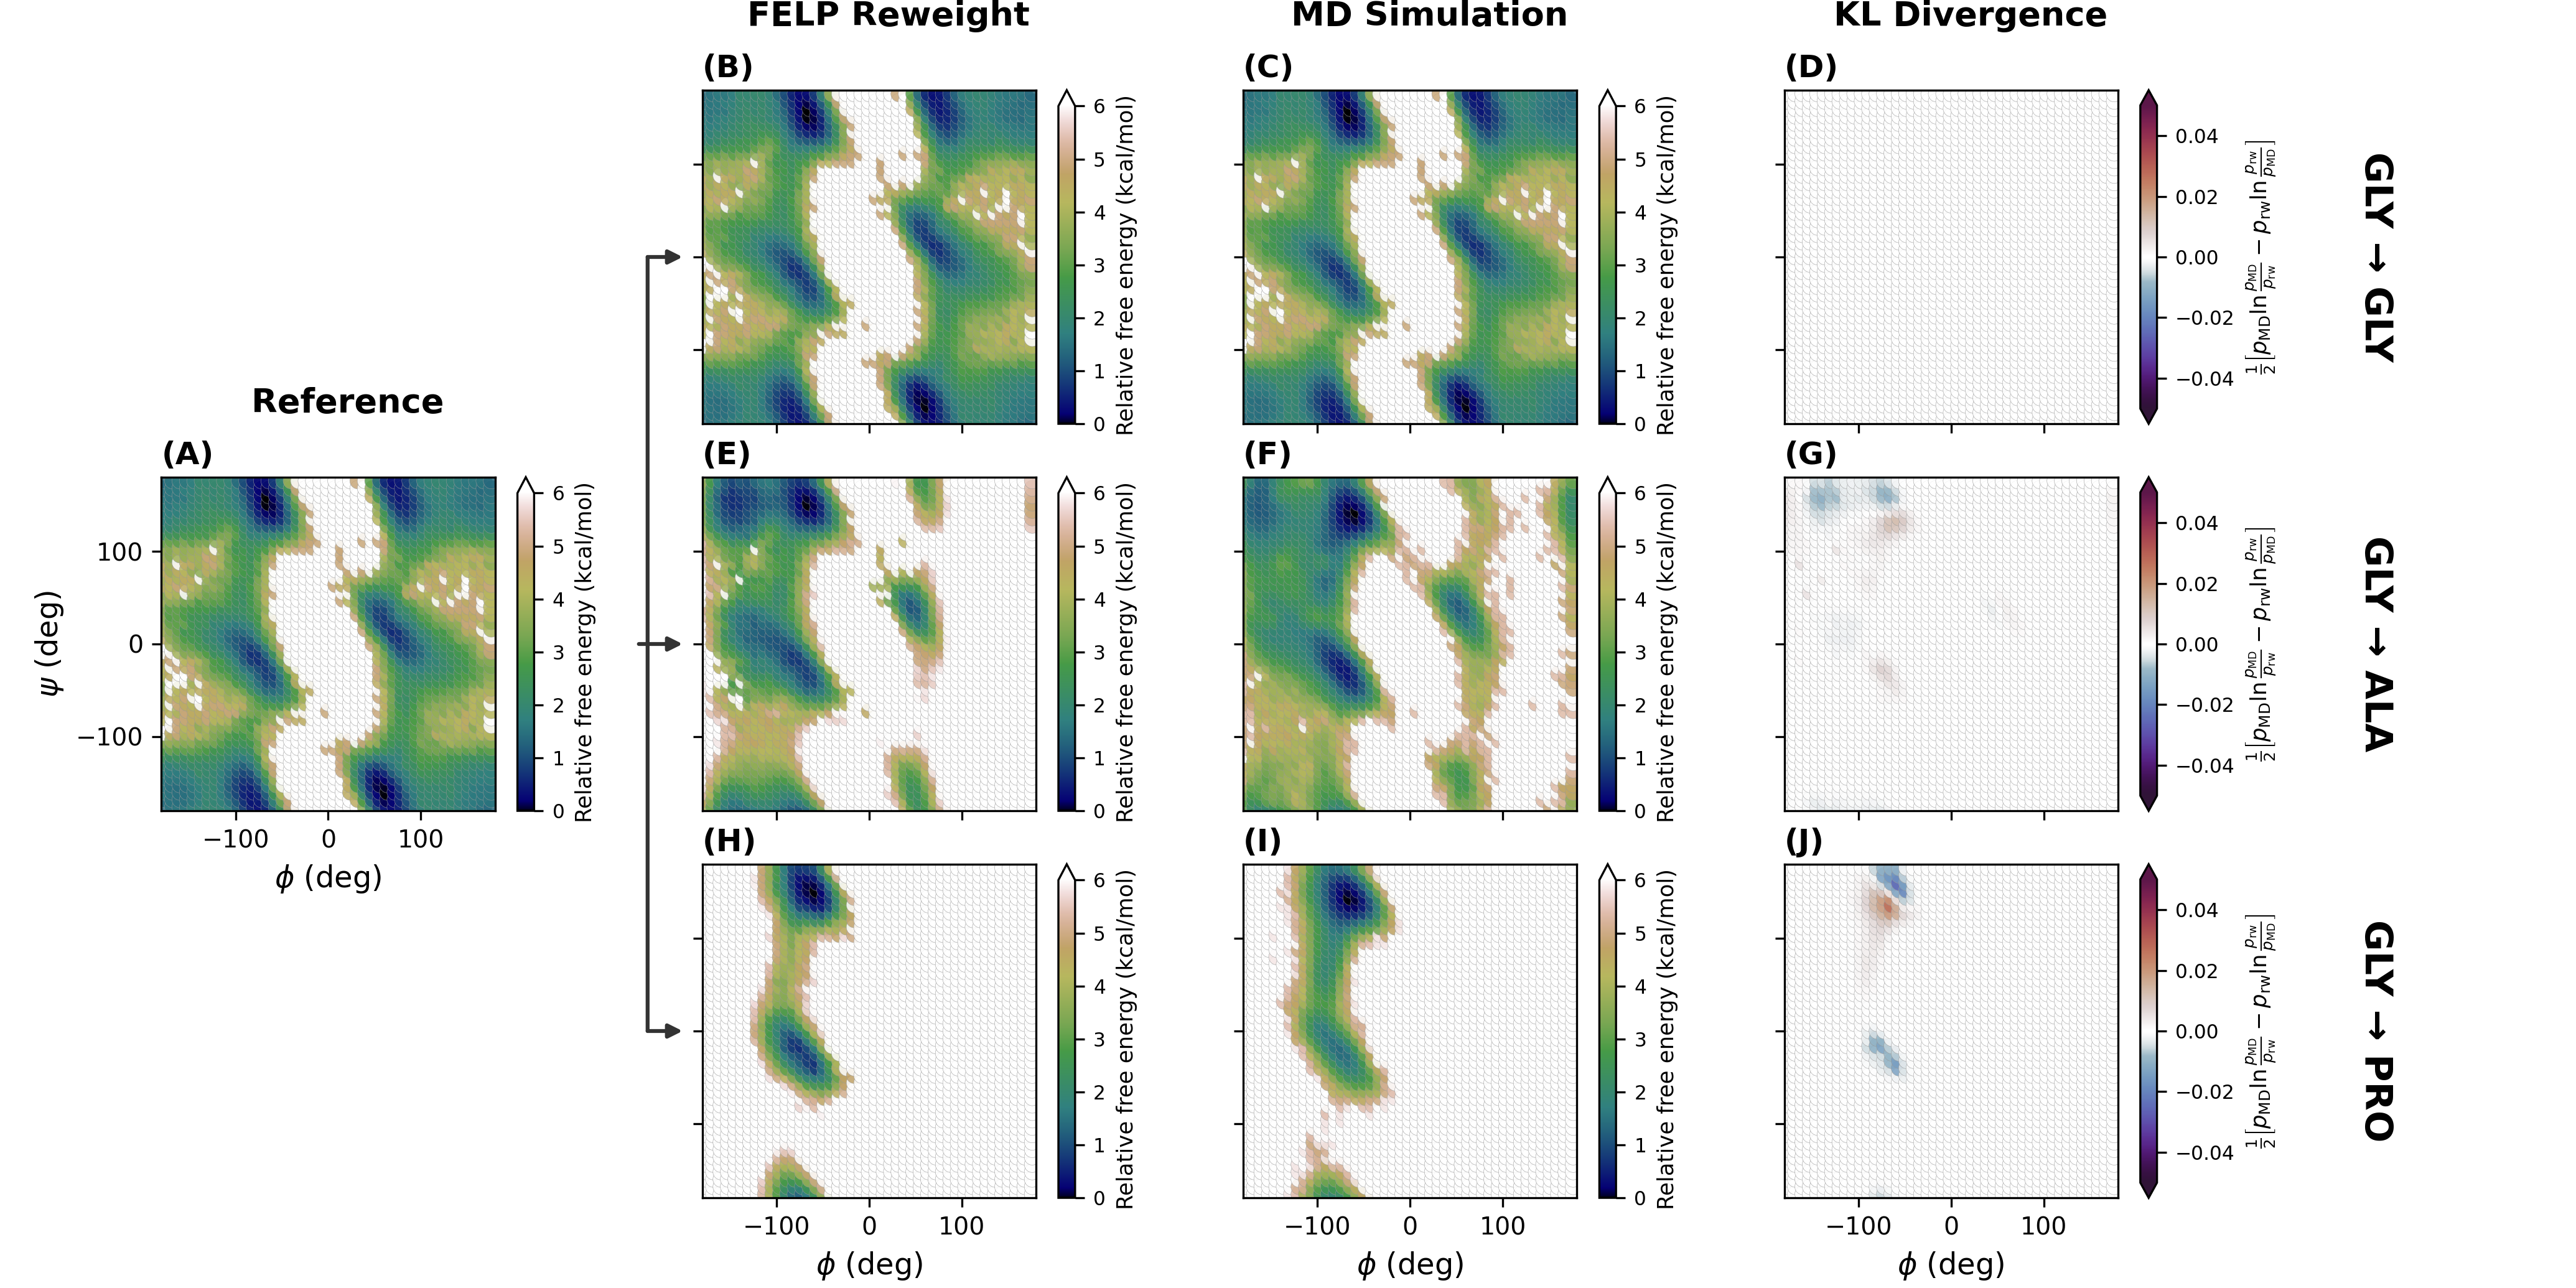
\includegraphics[width=\textwidth]{figures/GLY.rotation_mutations_composite.png}
		\caption{\textbf{FELP reweighting from a glycine dipeptide reference.} (A) Reference MD free energy landscape in $\phi/\psi$ space. The panels for GLY$\rightarrow$GLY (B--D), GLY$\rightarrow$ALA (E--G), and GLY$\rightarrow$PRO (H--J) show the FELP-reweighted landscape (left), independently sampled MD landscape (center), and KL divergence (right).}
		\label{fig:GlycineBenchmark}
	\end{figure*}
	
	\begin{figure*}[t]
			\centering
		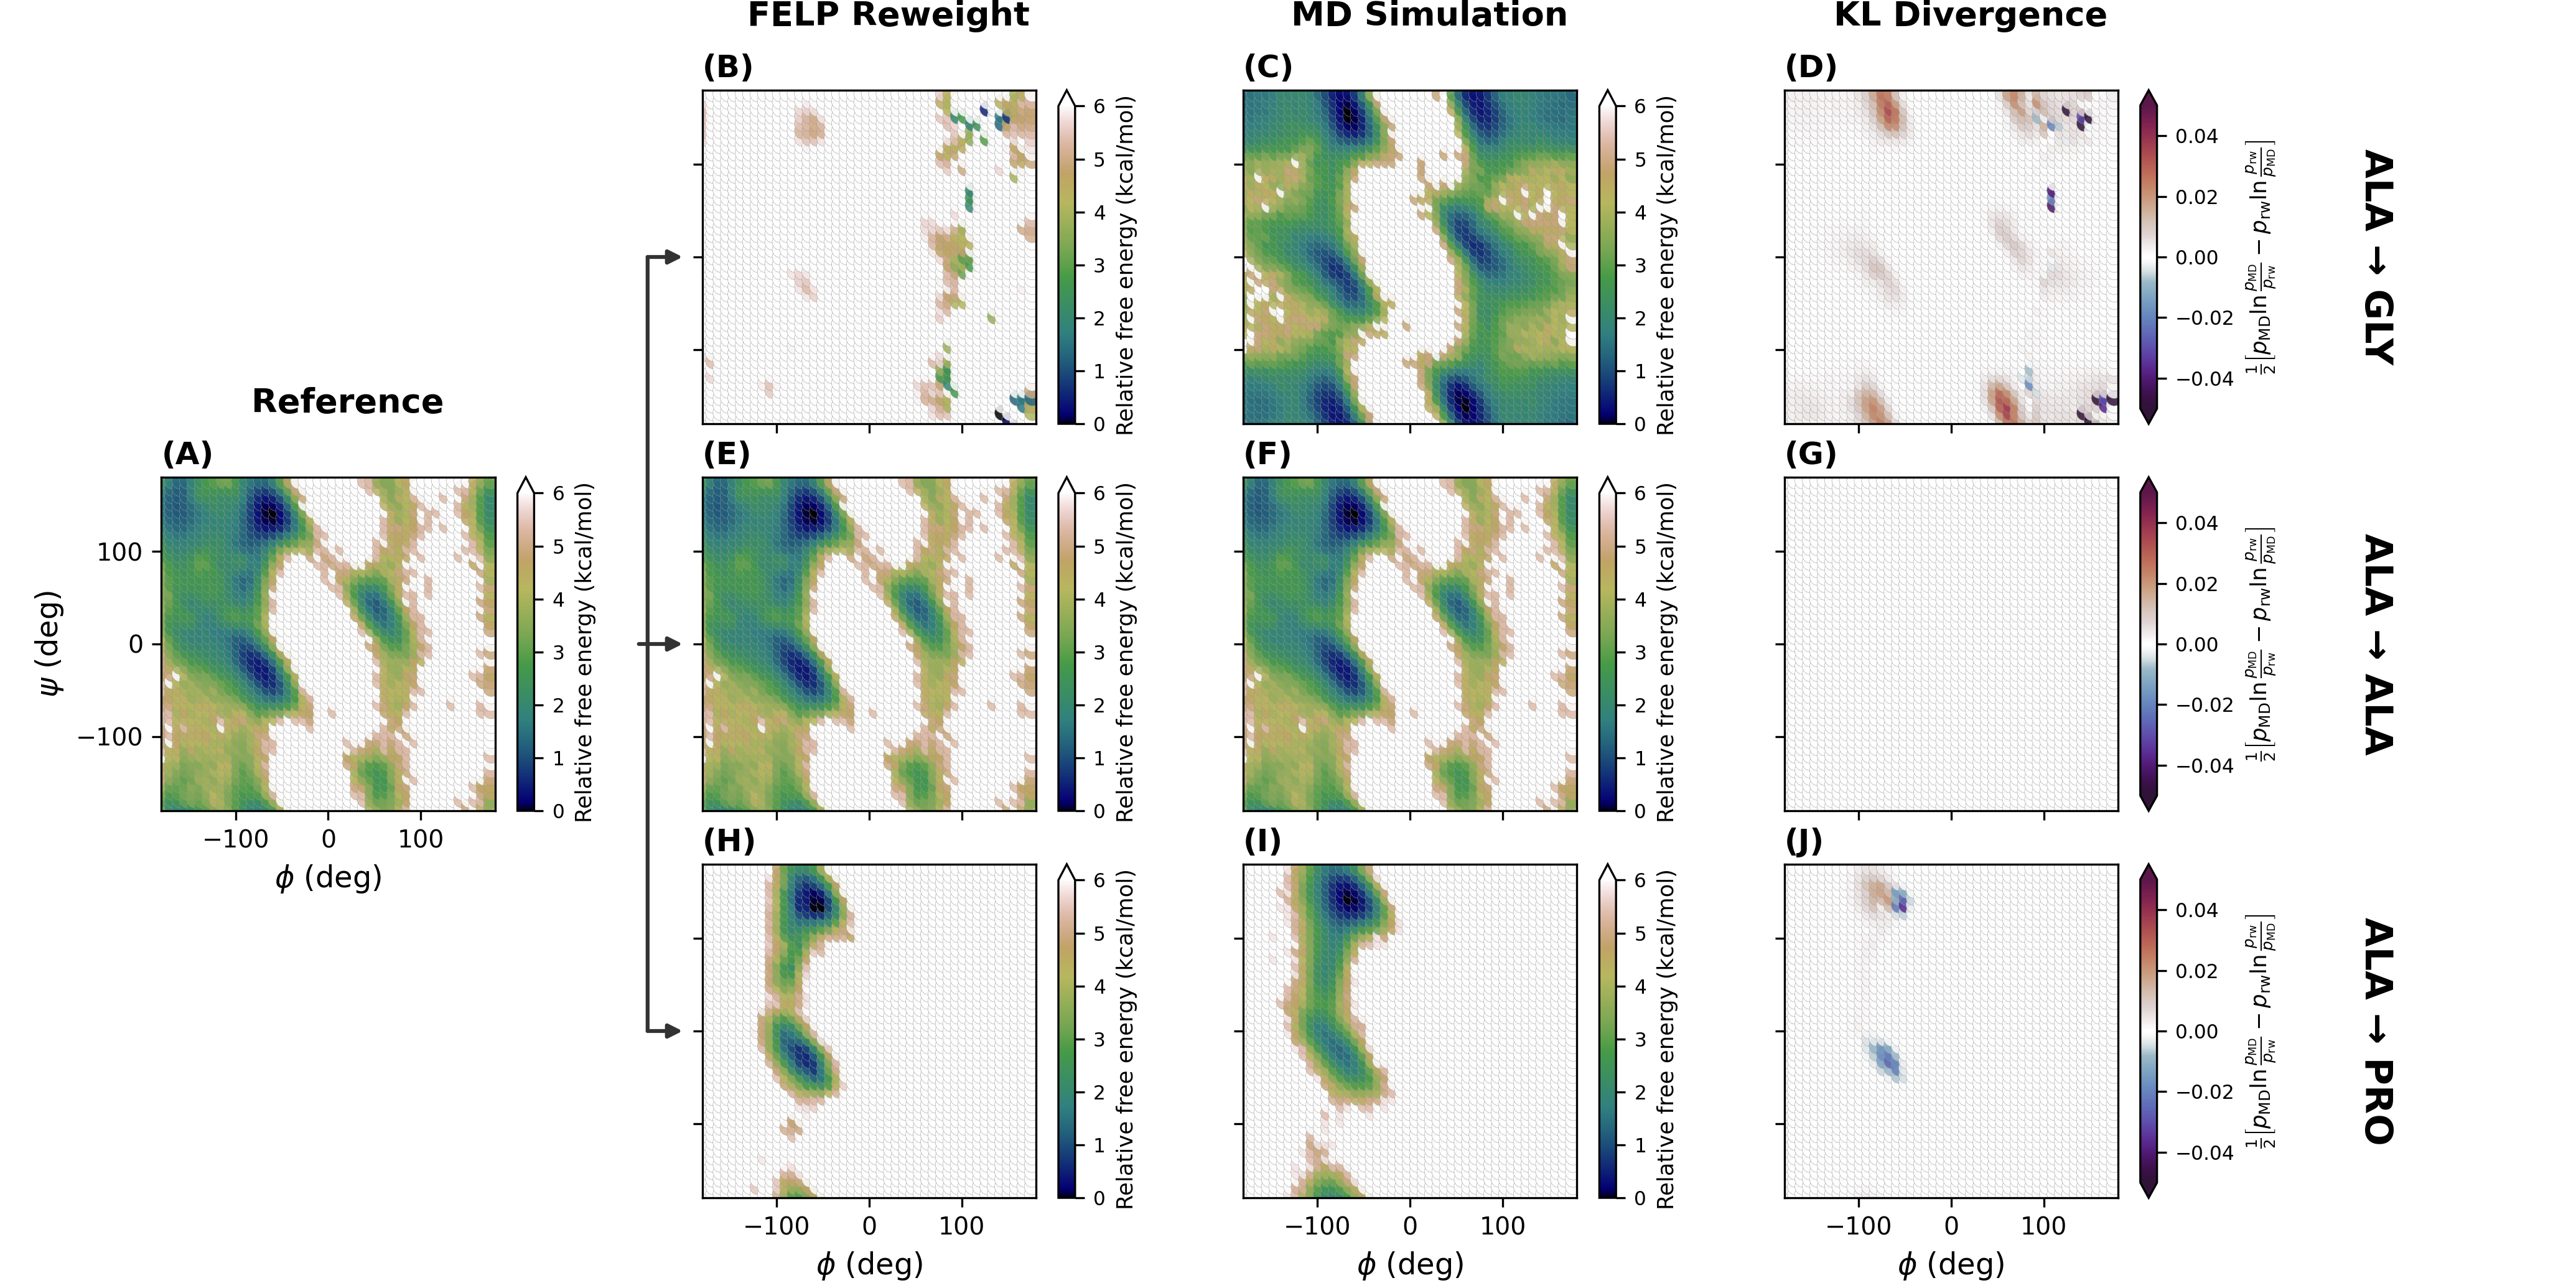
\includegraphics[width=\textwidth]{figures/ALA_rotation_mutations_composite.png}
		\caption{\textbf{FELP reweighting from an alanine dipeptide reference.} Layout as in \figrefcap{fig:GlycineBenchmark}. ALA$\rightarrow$GLY (B--D) fails to recover the broad glycine landscape because the required conformations are absent from the reference trajectory. ALA$\rightarrow$ALA (E--G) returns the identity. ALA$\rightarrow$PRO (H--J) succeeds because the proline landscape lies within the conformations sampled by alanine.}
		\label{fig:AlanineBenchmark}
	\end{figure*}
	
	\subsection{Overlap diagnostics quantify when reweighting fails}
	
	We next asked whether these success and failure modes could be identified from the reweighting statistics alone, without comparing against an independently sampled target landscape. For each GLY, ALA, and PRO reference ensemble, we reweighted to all 20 canonical amino acids and computed two diagnostics. The first is the target probability assigned to low-ESS states, nominally defined here as microstates with $\mathrm{ESS}_i < 10$, and the second is the maximum normalized frame weight \figrefp{fig:OverlapDiagnostics}.
	
	\begin{figure*}[t]
		\centering
		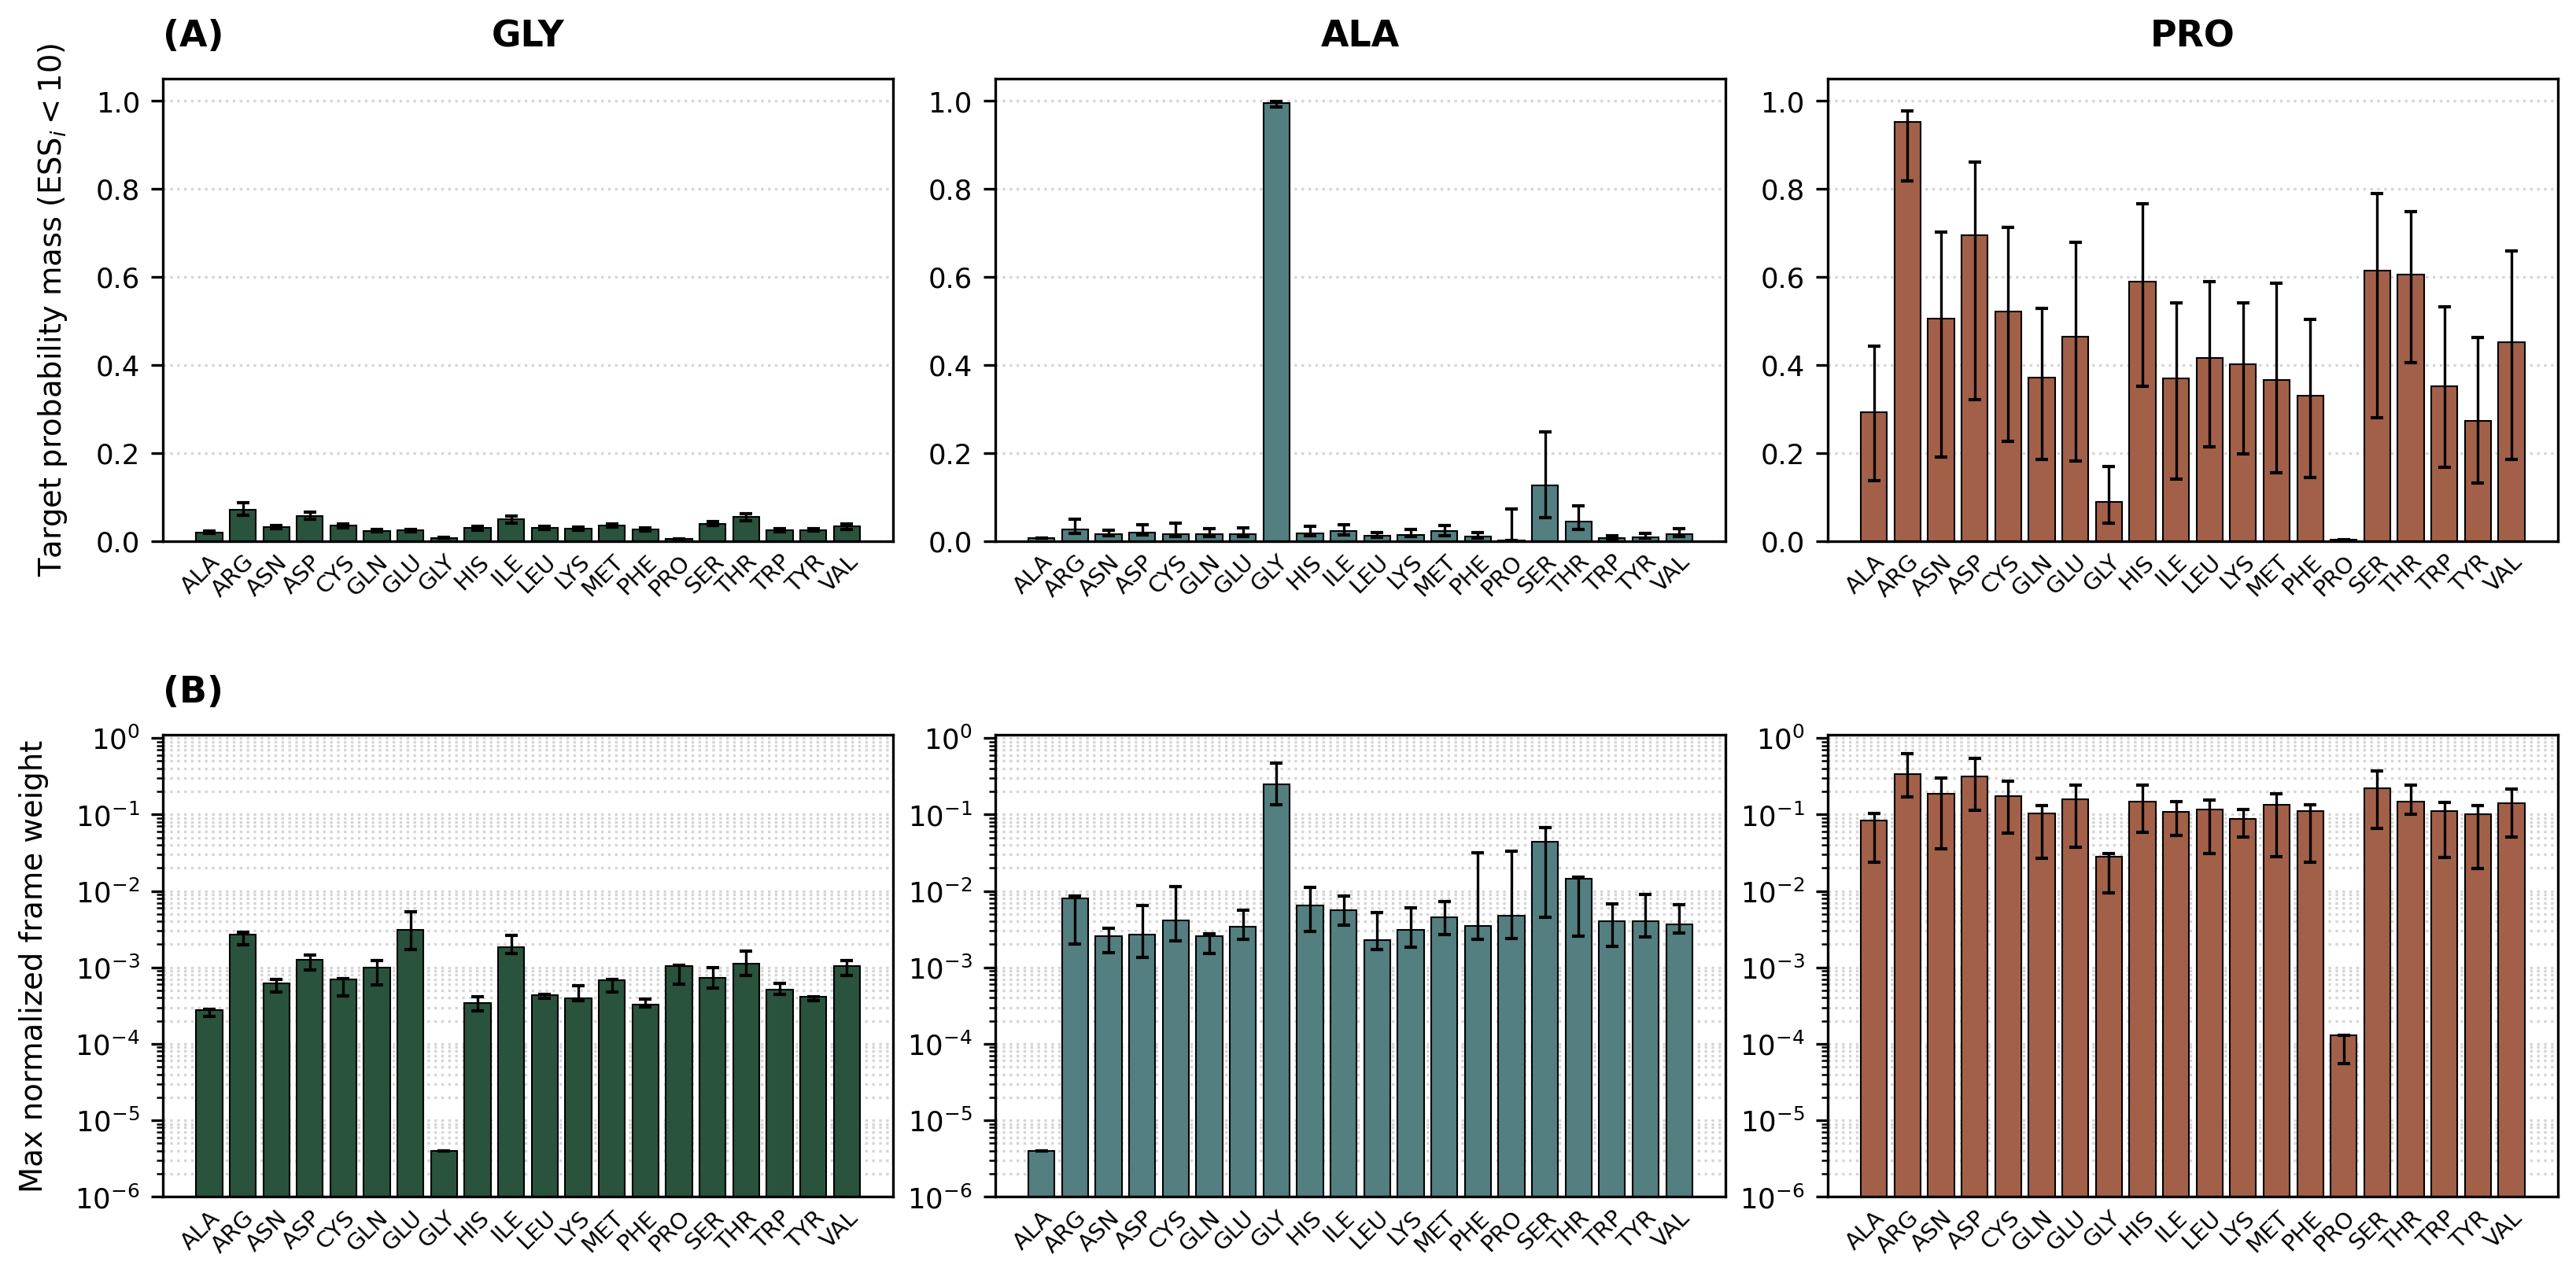
\includegraphics[width=\textwidth]{figures/overlap_diagnostics_two_panel.png}
		\caption{\textbf{Overlap diagnostics across reference ensembles.} (A) Fraction of target probability mass assigned to low-ESS states ($\mathrm{ESS}_i < 10$; $\mathcal{U}$, \eqnref{eq:unreliable_mass}) for all canonical amino acid targets from GLY, ALA, and PRO references. (B) Maximum normalized frame weight across the same perturbations. Error bars indicate bootstrap uncertainty across resampled evaluated frames.}
		\label{fig:OverlapDiagnostics}
	\end{figure*}
	
	The low-ESS mass remains small for all glycine-reference perturbations, consistent with the broad Ramachandran sampling of glycine \figrefp[A]{fig:OverlapDiagnostics}. The alanine reference shows the same pattern for most targets but fails sharply for ALA$\rightarrow$GLY, where nearly all target probability is assigned to low-ESS states. This diagnostic successfully identifies the missing-conformation failure observed visually in \figrefp[B--D]{fig:AlanineBenchmark} because the perturbation attempts to pull probability into the sparsely sampled tails of the alanine distribution. By contrast, the proline reference produces elevated low-ESS mass for most targets, reflecting the difficulty of using a conformationally restricted reference to predict broader amino-acid landscapes. PRO$\rightarrow$GLY, however, is an instructive exception. Deleting the pyrrolidine ring is a relatively smooth energetic perturbation within the conformations that proline already visits, so the reweighted probability is not concentrated in low-ESS states. One fundamental limitation of the diagnostic is that it cannot detect missing phase space if those conformations are never sampled by the reference.

	The maximum normalized frame weight provides a complementary view of the same overlap problem \figrefp[B]{fig:OverlapDiagnostics}. Glycine-reference perturbations are distributed over many frames, with maximum weights generally near $10^{-4}$--$10^{-3}$. Alanine-reference perturbations are also well-behaved except for targets such as glycine, where a small number of tail frames carry a disproportionate fraction of the reweighted probability. Proline-reference calculations show the largest frame-weight concentrations, in several cases approaching single-frame control of the local estimator. As with the low-ESS diagnostic, the comparatively modest frame-weight concentration for PRO$\rightarrow$GLY only indicates that the reweighting is statistically stable within the sampled proline conformations.

	Together, these data clarify the utility and limitations of internal overlap diagnostics for unidirectional reweighting. Metrics like $\mathcal{U}$ and maximum frame weight are necessary but not sufficient conditions for global landscape recovery. They reliably flag when a target landscape requires conformations that the reference rarely visits, as the estimator becomes starved for samples and dominated by statistical noise (e.g., ALA$\rightarrow$GLY). In these cases, the diagnostics prospectively warn that the predicted landscape is invalid and additional sampling is required. However, they cannot flag when a target landscape requires conformations that the reference never visits at all (e.g., PRO$\rightarrow$GLY), because unsampled regions contribute nothing to the estimator. Therefore, a favorable diagnostic guarantees that the prediction is statistically well-behaved within the reference bounds, but the user must still rely on chemical intuition or bidirectional sampling to ensure the reference ensemble was sufficiently broad to capture the relevant target biology. 
	
	\subsection{Chignolin}
	
	We next tested FELP on chignolin, a 10-residue $\beta$-hairpin miniprotein whose folding equilibrium depends on coordinated tertiary contacts rather than a single local backbone angle \cite{honda2004structure}. Wild-type chignolin is only marginally stable ($T_{\mathrm{m}}\approx315$~K). In contrast, the G1Y/G10Y variant of chignolin, CLN025, was designed to increase thermodynamic stability of the folded conformation ($T_{\mathrm{m}}\approx343$~K) while retaining the same hairpin topology \cite{honda2008jacs}. Circular dichroism and NMR place chignolin near half-folded at physiologically relevant temperatures. A two-state fit to the experimental melting curves gives $p_{\mathrm{fold}}\approx0.54$ for wild type at 310~K, whereas the same analysis gives $p_{\mathrm{fold}}\approx0.87$ for CLN025. NMR-based benchmarks similarly place wild-type chignolin near 60\% folded and CLN025 near 90\% folded at 300~K \cite{honda2004structure,honda2008jacs,fischer2024jctc}. Here, we projected the landscape onto two C$\alpha$ distances: (i) C$\alpha_1$--C$\alpha_{10}$, which reports on termini proximity, and (ii) C$\alpha_3$--C$\alpha_6$, which reports on turn formation. Together, these coordinates separate the compact folded basin from partially folded and extended conformations.
	
	Our 5~$\mu$s ff19SB/OPC reference trajectories substantially underfold both variants relative to experiment. Using the folded basin shown in \figref[A--D]{fig:ChignolinBenchmark}, wild-type chignolin has $p_{\mathrm{fold}}\approx0.12$ at 310~K, and the MD landscape spans both the compact folded basin and a broad set of extended conformations \figrefp[A]{fig:ChignolinBenchmark}. This underfolding is consistent with recent benchmark simulations. Fischer \textit{et al.}\ report $16\pm1\%$ natively folded for chignolin in substantially longer ff19SB/OPC trajectories analyzed with Markov state models, far below the experimental folded population \cite{fischer2024jctc}. Our MD simulations of CLN025 shift probability toward the folded basin while still sampling extended conformations \figrefp[B]{fig:ChignolinBenchmark}; its MD folded population is higher than wild type ($p_{\mathrm{fold}}\approx0.47$) but remains well below the experimental estimate of $p_{\mathrm{fold}}\approx0.87$.
	
	Reweighting improves these folded populations when the mutation is evaluated on an already sampled landscape. The CLN025$\rightarrow$WT calculation moves the wild-type estimate upward from the direct MD value ($p_{\mathrm{fold}}\approx0.12$) to $p_{\mathrm{fold}}\approx0.30$, closer to the experimental value of $0.54$ but still underfolded \figrefp[C]{fig:ChignolinBenchmark}. The WT$\rightarrow$CLN025 calculation starts from the broader wild-type reference and more strongly enriches the folded basin, giving $p_{\mathrm{fold}}\approx0.97$ compared with the experimental estimate of $0.87$ \figrefp[D]{fig:ChignolinBenchmark}. Thus FELP substantially improves the thermodynamic population estimates relative to direct ff19SB/OPC MD, with the strongest agreement in the WT$\rightarrow$CLN025 direction.
	
	We quantified these shifts by defining the folded basin as C$\alpha_1$--C$\alpha_{10}=4.0$--7.0~\AA\ and C$\alpha_3$--C$\alpha_6=5.5$--6.8~\AA\ (dashed boxes in \figref[A--D]{fig:ChignolinBenchmark}). Despite the absolute underfolding of the reference MD ensembles, the simulations recover the experimental sign and approximate magnitude of the CLN025 stabilization. The two-state experimental estimate gives $\Delta\Delta G_{\mathrm{fold}}\approx-1.0$~kcal~mol$^{-1}$, and the MD simulations give a similar value because both variants are shifted toward unfolded populations \figrefp[E, F]{fig:ChignolinBenchmark}. FELP recovers the same stabilizing direction and improves the absolute folded populations, but it overestimates the CLN025 stabilization, predicting CLN025 to be too stable by roughly 1.5~kcal~mol$^{-1}$. Interpreting this result requires separating force-field limitations in the reference ensemble from the additional approximation introduced by implicit-solvent mutation scoring. The former already compresses folded populations well below experiment in ff19SB/OPC, whereas the latter likely amplifies the terminal tyrosine stabilization because solvation contributions dominate folding thermodynamics in this small $\beta$-hairpin. Nevertheless, the chignolin benchmark shows that FELP can use an imperfect but structurally informative MD landscape to recover experimentally meaningful mutation-induced population shifts.
	
	\begin{figure*}[t]
	\centering
		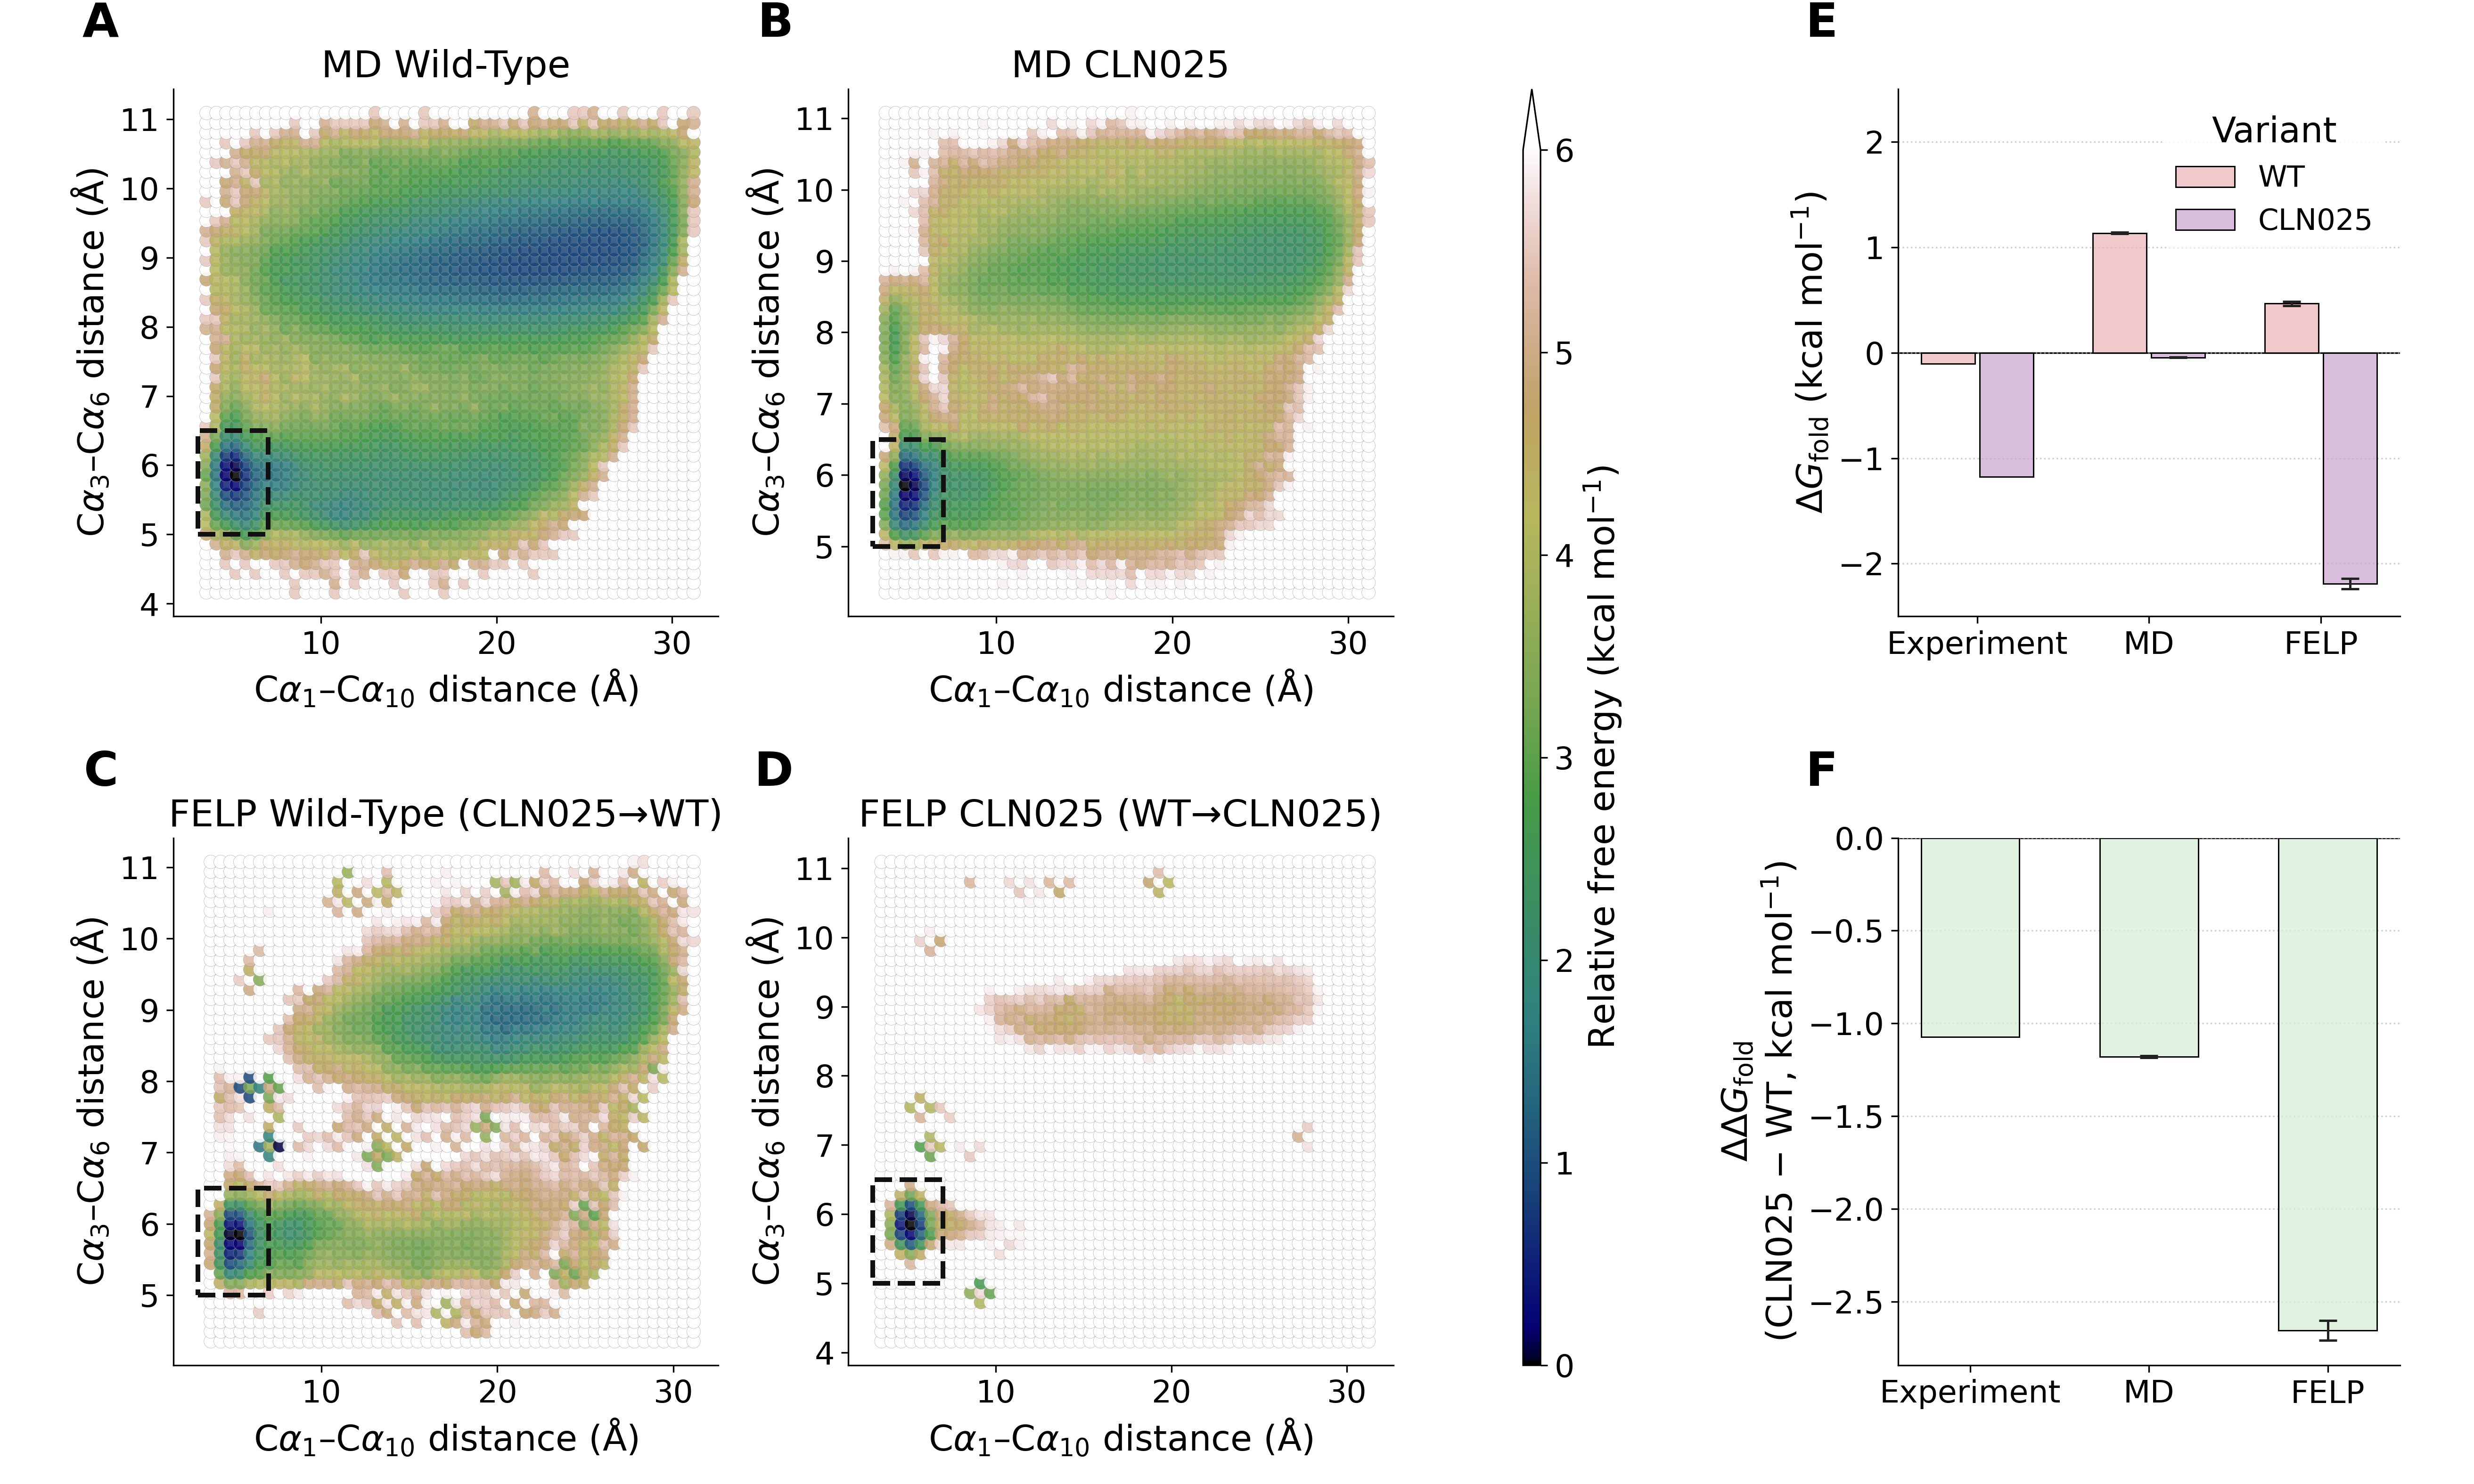
\includegraphics[width=\textwidth]{figures/chignolin_folding_landscape_figure.png}
		\caption{\textbf{FELP predicts mutation-induced folding shifts in chignolin.} (A, B) MD free energy landscapes for wild-type chignolin and CLN025 projected onto C$\alpha_1$--C$\alpha_{10}$ and C$\alpha_3$--C$\alpha_6$ distances. Dashed boxes indicate the folded basin. (C) FELP CLN025$\rightarrow$WT reweighted landscape. (D) FELP WT$\rightarrow$CLN025 reweighted landscape. (E) Folding free energies $\Delta G_{\mathrm{fold}}$ from experiment, MD, and FELP. (F) $\Delta\Delta G_{\mathrm{fold}}$ (CLN025 $-$ WT).}
		\label{fig:ChignolinBenchmark}
	\end{figure*}
	
	\subsection{T4 lysozyme}
	
	Finally, we applied FELP to T4 lysozyme, a larger protein system in which mutation alters the conformational landscape through hydrophobic core packing. The L99A substitution creates an internal cavity of approximately 150~\AA$^3$ \cite{eriksson1992t4} and is among the most extensively characterized cavity-creating mutations in structural biology \cite{morton1995t4}, with conformational exchange between ground and excited states observed by NMR relaxation dispersion \cite{mulder2001t4l,vallurupalli2016t4l}. We used L99A as the reference ensemble and reweighted toward wild type (A99L), projecting the result onto $\psi_{114}$, a Phe114 backbone dihedral reporting on helix~F dynamics near the cavity.
	
	\begin{figure}[t]
			\centering
		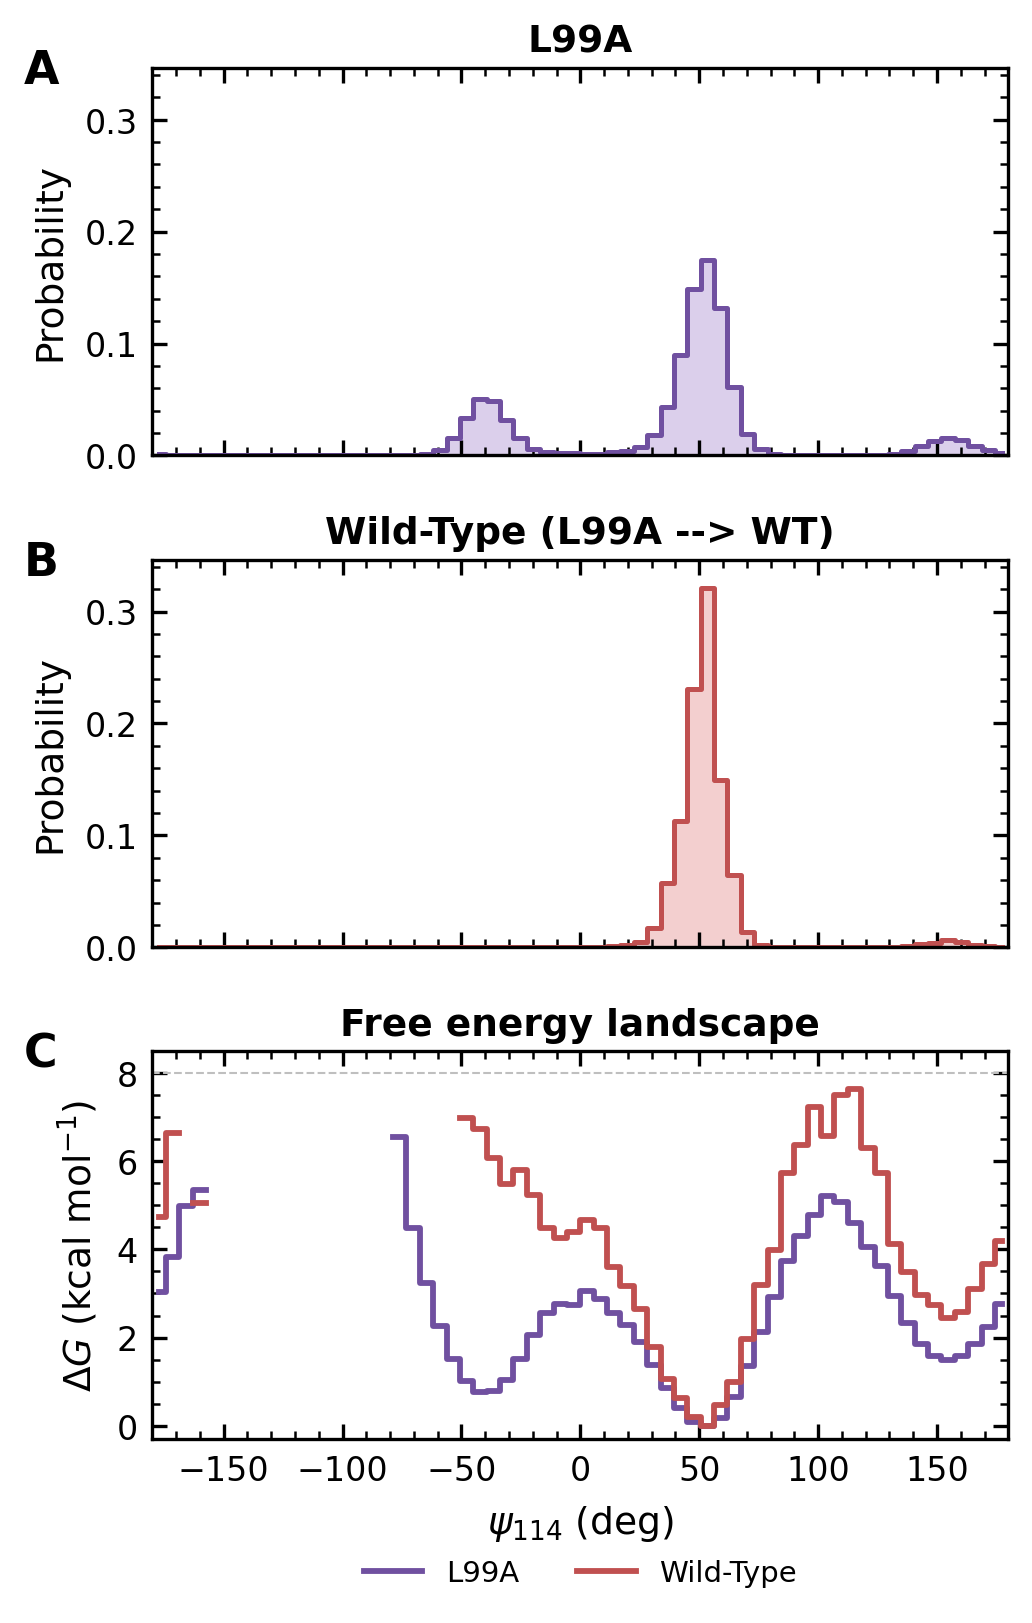
\includegraphics[width=\linewidth]{figures/t4_a99l_landscape_figure_3panel.png}
		\caption{\textbf{FELP predicts helix~F conformational redistribution upon cavity filling in T4 lysozyme.} (A) Reference L99A probability distribution over $\psi_{114}$. (B) FELP-reweighted wild-type (L99A$\rightarrow$WT) distribution. (C) Free energy landscapes for L99A (purple) and FELP-reweighted wild type (red).}
		\label{fig:T4LBenchmark}
\end{figure}
	The L99A reference distribution is dominated by a basin near $\psi_{114}\approx55^\circ$, but it also contains lower-probability excursions near $\psi_{114}\approx-40^\circ$ and near the periodic boundary \figrefp[A]{fig:T4LBenchmark}. Reweighting toward wild type further concentrates probability into the $\psi_{114}\approx55^\circ$ basin and strongly suppresses the secondary L99A populations \figrefp[B]{fig:T4LBenchmark}. The corresponding free energy projection shows the same trend. The wild-type landscape retains the same global minimum but raises the alternative regions of $\psi_{114}$ space relative to L99A \figrefp[C]{fig:T4LBenchmark}.
	
	This behavior is physically consistent with cavity filling. The L99A cavity allows for alternative helix~F packing arrangements, whereas restoring the bulky leucine side chain sterically restricts these excursions. This calculation highlights FELP's strength when the reference ensemble is conformationally broader than the target. Because the L99A simulation already samples the relevant extended phase space, reweighting toward wild type is statistically well-posed. FELP correctly identifies that the perturbation penalizes the minor basins and redistributes probability into the dominant, well-packed conformation.
	
	\section{Discussion}
	
	Understanding how mutations in proteins alter their conformational free energy landscapes is central to interpreting allosteric mechanisms, predicting resistance phenotypes, and guiding protein engineering. However, converging a separate MD ensemble for every mutation of interest is prohibitively expensive. FELP addresses this by asking a narrower question. Given a well-sampled reference landscape, how does a chemical perturbation redistribute probability among the states already observed?
	
	FELP belongs to an emerging class of population-shift methods that reuse a reference conformational ensemble rather than resampling each perturbation from scratch. In ligand binding, implicit-ligand theory formalized how ligand interactions can reweight apo conformations to estimate binding thermodynamics and conformational selection \cite{minh2012implicit,nguyen2018implicit,schutte2015alchemy}. More recent discrete-state implementations make this idea practical for MSMs. For example, PopShift reweights ligand-free MSM states using empirical docking scores to predict ligand-induced population shifts \cite{smith2024popshift}. Related mutation-focused work has used peptide--MHC MSMs to reweight metastable macrostate populations for peptide variants \cite{abella2020msm}. FELP adapts the same population-shift principle generally to amino-acid mutations by replacing empirical state scores or coarse macrostate corrections with restrained FEP-style energy differences evaluated within microstates, and by reporting overlap diagnostics alongside the predicted population shift.
	
	Our dipeptide benchmarks demonstrate that FELP reliably recovers the perturbed landscape when the target conformational ensemble lies within the region sampled by the reference \figsrefcp{fig:GlycineBenchmark}{fig:AlanineBenchmark}. The self-perturbation controls confirm that the pipeline is stable, and the GLY$\rightarrow$ALA and GLY$\rightarrow$PRO results show that FELP can correctly predict the restriction of accessible Ramachandran space upon side-chain addition. The reverse transformation, ALA$\rightarrow$GLY, fails precisely because the target requires conformational basins absent from the reference ensemble. This failure is expected from the asymmetric overlap requirements of unidirectional reweighting and is correctly identified by the $\mathcal{U}$ diagnostic without access to a target simulation \figrefp{fig:OverlapDiagnostics}.
	
	The chignolin benchmark extends these overlap tests to a system where the conformational equilibrium depends on coordinated intramolecular contacts. The explicit-solvent reference trajectories underfold both chignolin variants relative to experiment, a known limitation of the ff19SB/OPC force field \cite{fischer2024jctc}. Despite this poor starting point, FELP correctly identifies that CLN025 is more stable than wild-type chignolin, and it shifts the absolute folded populations of both variants closer to experimental estimates. This improvement in absolute populations, however, must be interpreted carefully. Implicit-solvent scoring can introduce systematic biases relative to explicit-solvent reference ensembles, and the magnitude depends on the force field and GB model pairing \cite{nguyen2013gbneck2}. In this case, the implicit-solvent bias toward the folded state fortuitously counteracts the explicit-solvent model's bias toward the unfolded state. While this cancellation of errors recovers more accurate absolute populations, the solvent-model mismatch leads FELP to overestimate the relative $\Delta\Delta G_{\mathrm{fold}}$. Because the perturbation is evaluated with a different energy model than the reference simulation, the reweighted landscape reflects the combined physical approximations of both.
	
	A related practical limitation arises from the solvent model mismatch. Reference MD simulations in our benchmarks were performed in explicit OPC water, whereas FELP evaluates $\Delta U$ using implicit GBNeck2 solvent on stripped protein coordinates. This choice avoids the need for explicit solvent relaxation at each evaluated frame, which would substantially increase computational cost and reduce the practical advantage of the reweighting approach. However, it introduces a systematic approximation, as the $\Delta U$ values reflect the mutation's effect under implicit solvation rather than in the explicit-solvent environment of the reference trajectory. For small perturbations in well-packed protein cores, this mismatch may be modest; for perturbations that change solvent exposure or disrupt hydrogen-bonding networks, the implicit-solvent $\Delta U$ may diverge from the explicit-solvent value. For membrane proteins, this issue is compounded because evaluating stripped coordinates in bulk implicit solvent discards protein--lipid interactions, asymmetric electrostatics, and hydrophobic mismatch effects that were present in the explicit bilayer simulation. Extending FELP to mutations that engage lipids will therefore require either explicit-environment perturbation evaluation or benchmarked approximations that preserve the relevant membrane contributions. A potentially more tractable alternative may be to evaluate perturbations with membrane-aware implicit solvent models. Indeed, this is an area of development in Rosetta, including recent implicit membrane energy function benchmarks and extensions to non-planar membrane geometries \cite{alford2021membrane,samanta2024membrane,woods2024membrane}.
	
	In addition, the local Zwanzig estimator is inherited from FEP and carries the same phase-space overlap requirements as any exponential reweighting calculation. The global landscape estimate is obtained by applying these local perturbation factors across a reference state model. Our diagnostics (ESS, maximum frame weight, $\mathcal{U}$) formalize this requirement as a computable criterion that accompanies every prediction. When diagnostics are favorable, FELP can estimate mutation-induced population shifts at far lower cost than independently converging each perturbed ensemble. When diagnostics are unfavorable, the method provides direct evidence that the reference ensemble did not adequately sample the conformations needed for the proposed perturbation and that new sampling is required.

	The use of a unidirectional exponential average is not the only possible estimator for this state-local problem. Bidirectional estimators such as the Bennett acceptance ratio (BAR) or multistate estimators such as MBAR can reduce variance when samples from both end states, or from intermediate alchemical states, are available \cite{shirts2005comparison,shirts2008mbar}. Nonequilibrium switching or staged perturbation paths could also improve overlap within difficult microstates. These alternatives would trade additional simulation or energy-evaluation cost for reduced estimator variance. FELP uses the unidirectional form because it preserves the central screening use case, allowing many perturbations to be evaluated from a single reference ensemble without generating target trajectories. Future implementations could introduce intermediate-state evaluation selectively for microstates flagged by the overlap diagnostics.
	
	The most important conceptual limitation is that FELP estimates the perturbed distribution over the reference state space. It cannot discover conformational basins that the reference trajectory did not visit. In the present implementation, energies are computed after local mutation and restrained relaxation without extended equilibration or explicit treatment of large-scale solvent reorganization. FELP is therefore best understood as an estimator of how a perturbation biases existing conformations, not as a substitute for free energy calculations in cases where the mutation induces substantial structural reorganization beyond the scope of the reference ensemble.
	
	Nevertheless, these limitations define FELP's intended utility. A predicted redistribution is most useful when it occurs on a functional free energy surface, retains low unreliable target probability mass, and is derived from distributed frame weights. Under those conditions, FELP can prioritize mutation-induced population shifts for mechanistic follow-up at substantially lower cost than direct resimulation of every variant. Conversely, high $\mathcal{U}$, concentrated frame weights, or known environmental contributions that are absent from the perturbation model provide direct evidence that the result should be treated as a sampling or model-fidelity problem rather than as a mechanistic conclusion. Future development should address the solvent mismatch through explicit-solvent evaluation protocols or hybrid strategies that reintroduce solvent contributions selectively, and broader benchmarks on proteins with experimentally characterized conformational equilibria will further clarify the practical scope of the reweighting approximation.
	
	\section{Methods}
	
	\subsection{FELP workflow}
	
	The FELP workflow has four stages \figrefp{fig:FELPWorkflow}. First, a sampled reference ensemble is obtained for the system expected to contain the relevant conformational ensemble. In the present benchmarks this ensemble comes from explicit solvent MD simulations, but in general the requirement is a meaningful prior over reference states. The sampled configurations are summarized into microstates defined in a chosen collective variable space, such as a uniform $\phi/\psi$ grid, distances or other user-specified coordinates in an explicit JSON/YAML state file, or states imported from an exported MSM bundle.
	
	Second, each reference frame is assigned to a microstate. When raw-count priors are used, $\hat{\pi}_0(i)$ is the empirical fraction of assigned reference frames in state $i$. When a state file or MSM bundle contains trusted reference probabilities, FELP can instead normalize those loaded priors. For the purposes of our benchmark systems in this study, we made use of raw counts from our MD simulations as our priors.
	
	Third, FELP evaluates selected configurations within each state. The purpose of this stage is to estimate how a mutation changes the energy of each reference frame while keeping the comparison local to the microstate in which that frame was observed. For every frame, FELP prepares two branches from the same starting pose. The reference branch enforces the original residue identity, and the perturbed branch introduces the target amino acid(s). We measure the configured collective variables in the reference pose and convert those values into restraint targets. Strong harmonic restraints in the CV definition space are applied identically to both branches, so that each evaluated structure remains pinned to the assigned conformational coordinates while the mutation is introduced and scored.
	
	Local structure preparation was performed with PyRosetta \cite{chaudhury2010pyrosetta} Cartesian FastRelax using the constrained ref2015 score function \cite{alford2017ref2015}. Backbone-dihedral CVs are enforced as Rosetta dihedral constraints and distance CVs as atom-pair constraints with narrow harmonic widths. In addition to these CV restraints, FELP exposes separate controls over which internal degrees of freedom may relax. By default, FastRelax was run for five cycles with Cartesian minimization, rigid-body jumps disabled, and design disabled. Sidechain repacking is restricted to a mobile residue set selected by the mobility policy; all other side chains are held fixed through the task factory. Unless a benchmark specified otherwise, only the mutated residue side chain is mobile. These mobility settings determine how much additional relaxation is permitted around the pinned CV coordinates and therefore trade structural flexibility for computational cost; they do not replace the CV restraints themselves.
	
	After Rosetta preparation, both branches are converted for evaluation in OpenMM \cite{eastman2017openmm} with the ff14SB sidechain-only protein force field \cite{maier2015ff14sb} and GBNeck2 implicit solvent \cite{nguyen2013gbneck2}. The base CV restraints are re-imposed as harmonic torsion and distance potentials, atoms outside the mobile set are fixed by zero mass, and each structure is energy-minimized until convergence. FELP records the energy difference $\Delta U_{ij}=U_1(x_{ij})-U_0(x_{ij})$ for each evaluated frame and excludes failed or non-finite frames from reweighting.
	
	Fourth, FELP aggregates frame-level Boltzmann factors into state-level reweighting factors. Perturbed probabilities follow \eqnref{eq:sample_reweighting}, with local factors $f_i$ computed from the in-state average of $w_{ij}=\exp[-\beta(\Delta U_{ij}-s)]$. To regularize noisy local estimates before normalization, we applied neighbor pooling across cardinal directions on the assignment grid, with the blending strength $\tau$ selected by the L-curve criterion described in \textbf{Theory}.

	\textbf{Dipeptide FELP settings.} Dipeptide mutations used residue~2 as the perturbation site and a $45\times45$ $\phi/\psi$ grid for assignment. The $\phi$ and $\psi$ angles of residue~2 were restrained in both Rosetta and OpenMM using a force constant of 100,000. No distance restraints or extra Rosetta-only backbone restraints were used. The default target-only mobility policy was used, so only the target side chain was repacked and minimized.

	\textbf{Chignolin FELP settings.} Chignolin CLN025$\rightarrow$WT calculations mutated residues 1 and 10 simultaneously (Y1G/Y10G) and used automatic microstates built from two distance CVs: C$\alpha_1$--C$\alpha_{10}$ and C$\alpha_3$--C$\alpha_6$. These distances were the base restraints in both stages. In Rosetta they were applied as atom-pair harmonic constraints with $\sigma=0.001$~\AA; in OpenMM they were applied as harmonic bond restraints with force constant 1,000,000. The Rosetta preparation stage also included Rosetta-only $\phi/\psi$ restraints on residues 1, 2, 9, and 10, using force constant 25,000 and a 15$^\circ$ tolerance for validation. Mobility used a sequence window of one residue around each mutation site with backbone and side-chain motion enabled, so residues 1--2 and 9--10 were mobile. An identical protocol was used for the WT$\rightarrow$CLN025 (G1Y/G10Y) calculation.

	\textbf{T4 lysozyme FELP settings.} T4 lysozyme L99A$\rightarrow$WT calculations used automatic microstates along $\psi_{114}$. The $\psi_{114}$ dihedral was the base restraint in both Rosetta and OpenMM, with force constant 10,000 during Rosetta preparation and 1,000,000 during OpenMM minimization. Rosetta preparation also applied Rosetta-only $\phi/\psi$ restraints to residue~99 with force constant 25,000 and a 15$^\circ$ validation tolerance. The mobile set was limited to the mutated residue, so only the residue~99 sidechain was mobile.
	
	\subsection{Reference simulations and trajectory processing}
	
	\textbf{Molecular dynamics simulations.} Except where specified otherwise below, reference ensembles were generated with explicit-solvent molecular dynamics using AMBER~24 \cite{case2025amber} and the GPU-accelerated \texttt{pmemd.cuda} engine. Proteins were parameterized with the ff19SB force field \cite{tian2020ff19sb} and solvated in orthorhombic periodic boxes of OPC water \cite{izadi2014opc}. Systems were neutralized with Na$^+$ or Cl$^-$ counterions using the monovalent ion parameters of Joung and Cheatham \cite{joung2008ions}. Simulations used periodic boundary conditions, the particle mesh Ewald method for long-range electrostatics with a 12.0~\AA\ real-space cutoff, SHAKE constraints on solute bonds involving hydrogen \cite{ryckaert1977shake}, and SETTLE constraints on water \cite{miyamoto1992settle}.  Hydrogen mass repartitioning (HMR) was applied to non-solvent atoms with ParmEd. We sequentially minimized solvent, solute, and the full system with 500 steps of steepest-descent minimization followed by 2,000 steps of conjugate-gradient minimization in each stage. Systems were heated from 10~K to 100~K in the canonical (NVT) ensemble for 1.0~ns and then to 310~K in the isothermal--isobaric (NPT) ensemble at 1~bar using a Monte Carlo barostat and isotropic volume scaling over an additional 1.0~ns. These two stages of heating were repeated as needed until the system was stable at 1~bar and 310~K. Production used a Langevin thermostat with collision frequency $\gamma = 1.0~\mathrm{ps}^{-1}$ at 310~K and a 4.0~fs timestep. Trajectory snapshots were saved every 10~ps. 
	
	\textbf{Dipeptides.} Capped dipeptide structures (ACE--X--NME) were built with \texttt{tleap}. Each dipeptide was solvated with a 20~\AA\ padding of OPC water. Production simulations of 2500~ns were performed for each dipeptide.
	
	\textbf{Chignolin.} Initial structures for wild-type chignolin and CLN025 were built in an extended conformation from sequence using \texttt{tleap}. The wild-type sequence was specified as \texttt{NGLY TYR ASP PRO GLU THR GLY THR TRP CGLY}. CLN025 was built similarly using the corresponding G1Y/G10Y sequence. Each system was solvated with a 15~\AA\ padding of OPC water. Reference trajectories were generated using the general MD protocol above. Production simulations of 5000~ns were performed for each system.
	
	\textbf{T4 lysozyme L99A.} Five X-ray structures capturing diverse starting states of T4 L99A lysozyme (PDB IDs: 4W52, 4W53, 4W54, 4W57, 4W59) were obtained and prepared by extracting chain A, retaining the first model, resolving non-canonical modified residues, and removing experimental artifacts. Systems were prepared with \texttt{tleap} using 12~\AA\ solvent padding. Production simulations were carried out for 5000~ns from each starting state.
	
	\subsection{Diagnostics and quality control}
		
	Before state-level factors $f_i$ are computed, FELP applies optional by-state quality control to the in-state Boltzmann weights. For each microstate, in-state weights are built from $\Delta U_{ij}$, and the upper-tail Pareto shape $k$ of the weight distribution is estimated with a PSIS-style rule \cite{vehtari2024psis}. A state is flagged when $k$ exceeds a sample-size-dependent reliability threshold. When frame exclusion is enabled, flagged states enter an iterative loop. First, the highest-weight frame is removed, then diagnostics are recomputed, and the loop continues until the state is no longer flagged or the configured per-state exclusion cap is reached. Local Zwanzig factors and $\mathrm{ESS}_i$ are then computed from the remaining frames only.
	
	Validity is summarized using \eqnref{eq:unreliable_mass} and its implementation extension,
	\begin{equation}
		\mathcal{U} =
		\sum_i \hat{\pi}_1(i)\,
		\mathbf{1}\{\mathrm{ESS}_i < \epsilon_i \; \mathrm{or}\; q_i = 1\},
	\end{equation}
	where $\epsilon_i=\max(5,\,0.1\,n_i)$ with $n_i$ the number of evaluated frames in state $i$, and $q_i=1$ when by-state diagnostics identify dominant-frame control of the local average (including states that remain flagged after frame exclusion). The run summary also records per-state $\mathrm{ESS}_i$, maximum normalized frame weights, and the target probability carried by QC-flagged states.
	
	\section{Code and Data Availability}
	
	The FELP source code and associated sample runtime scripts are freely available under an MIT license at \url{https://github.com/bpbrownlab/felp}.
	
	\section{Author Contributions}
	
	B.P.B. conceived the study. T.E.M. and B.P.B. wrote the code, designed the experiments, performed the simulations, conducted the analyses, interpreted the results, and wrote the manuscript.
	
	\section{Disclosures}
	
	B.P.B. is an advisor for Septagen Pharmaceuticals.
	
	\section*{Acknowledgments}
	This work was supported by the NIH (DP1DA058349). The authors thank members of the Center for AI in Protein Dynamics and the Department of Pharmacology at Vanderbilt University for helpful discussions.
	
	
	\bibliography{references}

\end{document}
